\documentclass[]{article}
\usepackage{geometry}
\geometry{margin=1in}

\usepackage{booktabs}
\usepackage{wrapfig}

\usepackage{graphicx}
\usepackage{amsmath,amsfonts,amssymb}
\usepackage{listings}

\usepackage{systeme}

%opening
\title{Layout and Proportionality Calculations for Rectilinear Effect Sensors in 6DOF Manipulator}
\author{David Wright}

\begin{document}
	
	\maketitle
	
	%\begin{abstract}
	
	%\end{abstract}
	
	\section{Background}

\begin{wrapfigure}{r}{0.25\textwidth}
	\begin{center}
		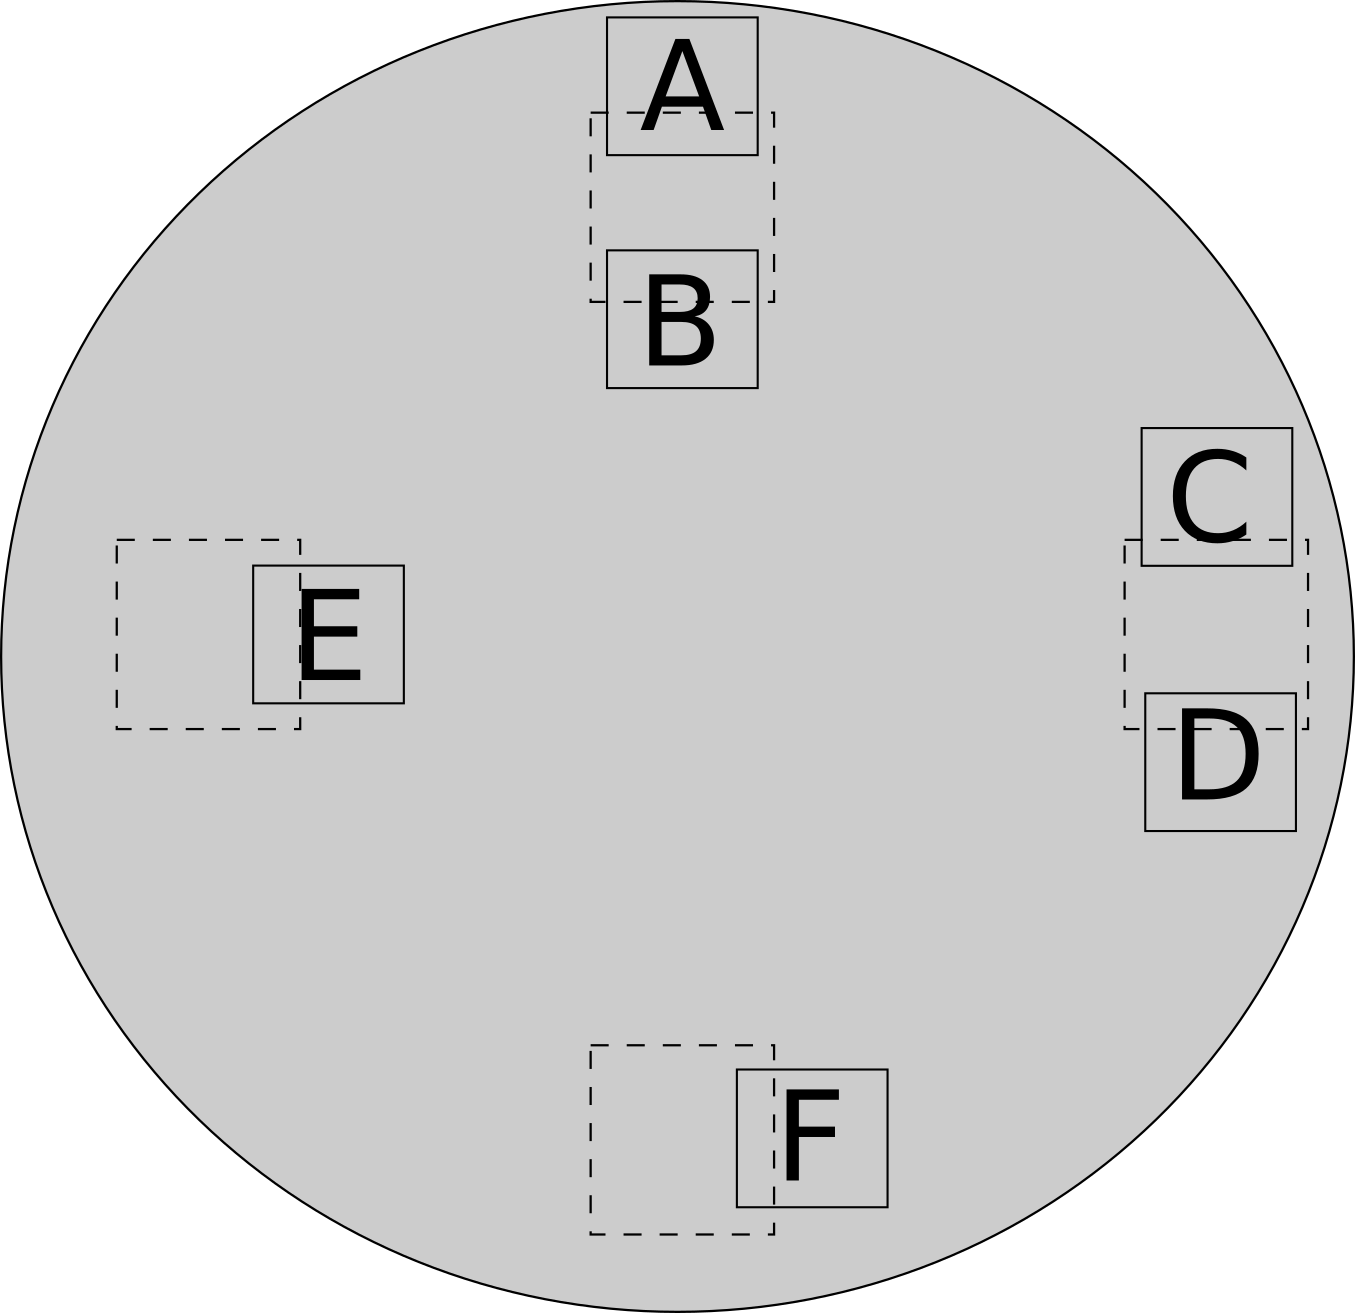
\includegraphics[width=0.23\textwidth]{layout.png}
	\end{center}
	\caption{Proposed 6-sensor rectilinear layout.}
	\label{fig:ProposedLayout}
	
\end{wrapfigure}
	RepRapPro recently shared a concept for a 6DOF manipulator using three pairs of hall effect sensor arranged at 120 degrees around a circular base. The kinematics of this map the six sensors to the 6 degrees of freedom of the controller. Given my preference for more simple software mapping between sensors and intended input, I propose the following rectilinear sensor layout.

	\section{Proposed Design}
	
	The proposed design uses 6 sensors arranged in pairs or alone at the cardinal points of the control puck base. Dashed lines indicate location of the magnet in the upper moving component. Sensors E and F do not have paired sensors, as the analysis below demonstrates their redundancy. 
	
	The mapping of sensor inputs to translation (T) and rotation (R) is given by the following proportionality matrix. 
		\[
	\begin{bmatrix}
		T_x \\
		T_y \\
		T_z \\
		R_x \\
		R_y \\
		R_z 
	\end{bmatrix} =
	\begin{bmatrix}
		-1 & -1 & -1 & -1 &  1 & 1\\
		1 & -1 & 1 & -1 &  -1 & -1 \\
		-1 & -1 & -1 & -1 &  -1 & -1 \\
		1 & 1 & 0 & 0 & 0 &  -1 \\
		0 & 0 & 1 & 1 &  -1 & 0 \\
		-1 & -1 & 1 &  -1 & -1 & 1 \\
	\end{bmatrix}
	\begin{bmatrix}
		A \\
		B \\
		C \\
		D \\
		E \\
		F \\
	\end{bmatrix}
	\]

	This conversion would just provide the relative proportions of each motion. Scaling to reasonable inputs can be done after this step. 

	\section{First Draft Design and Analysis}
	\begin{wrapfigure}{r}{0.2\textwidth}
	\begin{center}
		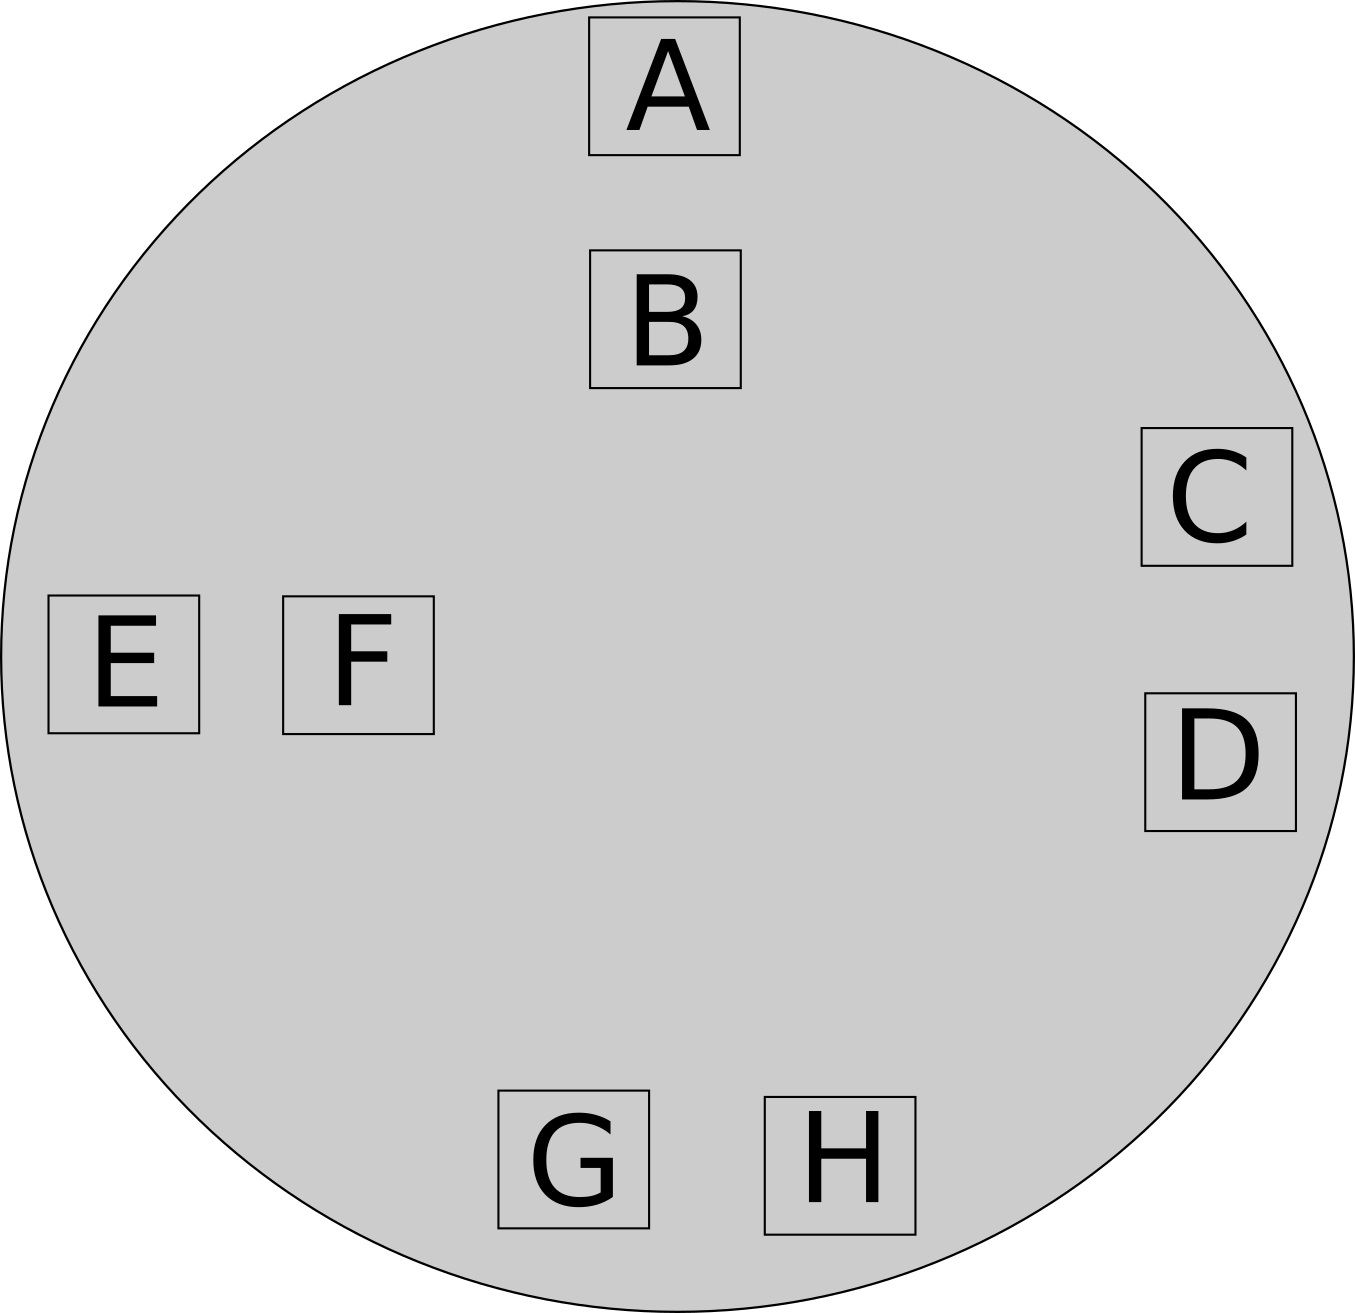
\includegraphics[width=0.18\textwidth]{layout_v1.png}
	\end{center}
	\caption{Version 1 of the rectilinear layout concept using 8 sensors.}
	\label{fig:LayoutV1}
	\end{wrapfigure}	
	
	The initial design used eight sensors, using pairs at the cardinal points of the circle. The intent was that for both x and y axes, there was a pair of sensors to detect translation and rotation. I assumed that the two additional sensors could be incorporated into the analysis for noise reduction.
	
	To map sensor inputs to desired output, I considered the effect of each direction separately on each sensors response, creating a linear set of equations, shown below. For a given 

	\begin{center}
	\[
		\systeme*{Translate_x=-A-B-C-D-E+F-G+H,
	Translate_y=A-B+C-D-E-F-G-H, 
	Translate_z=-A-B-C-D-E-F-G-H, 
	Rotate_x=A+B+0\cdot C+\cdot D + 0\cdot E + 0\cdot F - G - H, 
	Rotate_y=0\cdot A + 0\cdot B + 0\cdot C - E - F + G + H, 
	Rotate_z=-A-B+C-D-E-F-G+H}
\]		
	\end{center}

	This system of equations converts nicely into a linear algebra conversion, as given below.
	\[
	\begin{bmatrix}
	T_x \\
	T_y \\
	T_z \\
	R_x \\
	R_y \\
	R_z 
	\end{bmatrix} =
	\begin{bmatrix}
		-1 & -1 & -1 & -1 & -1 & 1 & -1 & 1\\
		1 & -1 & 1 & -1 & -1 & -1 & -1 & -1 \\
		-1 & -1 & -1 & -1 & -1 & -1 & -1 & -1 \\
		1 & 1 & 0 & 0 & 0 & 0 & -1 & -1 \\
		0 & 0 & 1 & 1 & -1 & -1 & 0 & 0 \\
		-1 & -1 & 1 & -1 & -1 & -1 & -1 & 1 \\
	\end{bmatrix}
	\begin{bmatrix}
		A \\
		B \\
		C \\
		D \\
		E \\
		F \\
		G \\
		H
	\end{bmatrix}
	\]

	This simplification shows that both inputs E and G are constantly -1 or is not used. From this it follows that they are redundant sensors and not needed for full 6DOF manipulation. 
	
\end{document}